%%%%%%%%%%%%%%%%%%%%%%%%%%%%%%%%%%%%%%%%%%%%%%%%%%%%%%%%%%%%%%%%%%%%%%%%%%%%%%
%%%%%%%%%%%%%%%%%%%%%%%%%%%%%%%%%%%%%%%%%%%%%%%%%%%%%%%%%%%%%%%%%%%%%%%%%%%%%%
%%
%% Dokumentácia k druhému projektu pre predmet IZP.
%%
%% Šablona dokumentácie od Davida Martinka.
%%%%%%%%%%%%%%%%%%%%%%%%%%%%%%%%%%%%%%%%%%%%%%%%%%%%%%%%%%%%%%%%%%%%%%%%%%%%%%
%%%%%%%%%%%%%%%%%%%%%%%%%%%%%%%%%%%%%%%%%%%%%%%%%%%%%%%%%%%%%%%%%%%%%%%%%%%%%%
\documentclass[12pt,a4paper,titlepage,final]{article}

% slovencina a fonty
\usepackage[slovak]{babel}
\usepackage[utf8]{inputenc}
% balicky pre odkazy
\usepackage[bookmarksopen,colorlinks,linkcolor=black,urlcolor=black,unicode]{hyperref}
\usepackage{url}
% obrazky
\usepackage{graphicx}
\usepackage{picture}
% velkost stranky
\usepackage[top=2.5cm, left=1.5cm, text={18cm, 25cm}]{geometry}
% lepsie tabulky
\usepackage{tabularx}
\usepackage{float}
\restylefloat{table}

\begin{document}

% titulná strana
\def\author{Ivan Ševčík}
\def\email{xsevci50@stud.fit.vutbr.cz}
\def\projname{Hra Breakout}
\begin{titlepage}

% \vspace*{1cm}
\begin{figure}[!h]
  \centering
  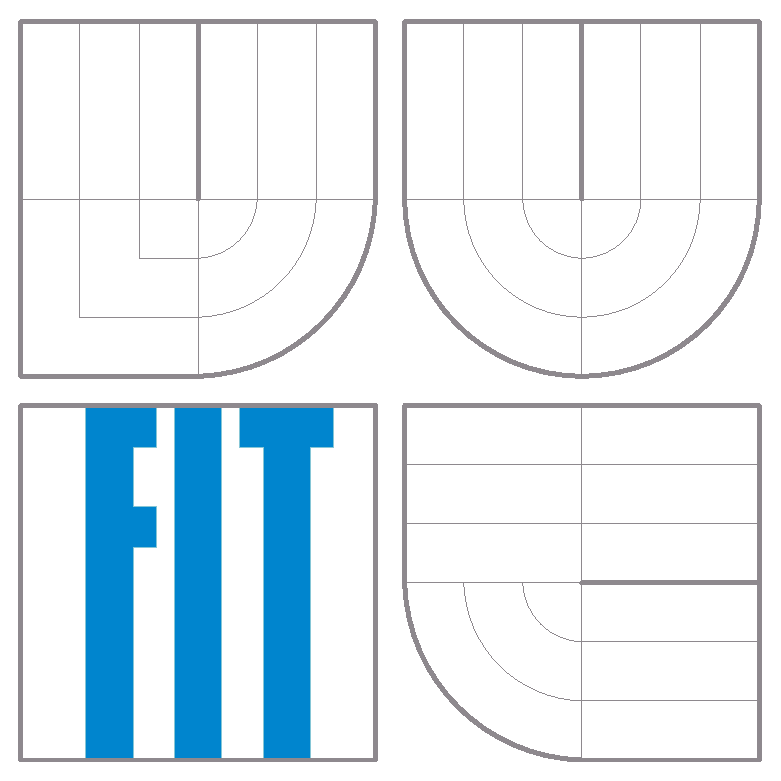
\includegraphics[height=5cm]{img/logo.eps}
\end{figure}

\vfill

\begin{center}
\begin{Large}
Dokumentácia k projektu pre predmet IVH\\
\end{Large}
\bigskip
\begin{Huge}
\projname\\
\end{Huge}
\begin{large}
\end{large}
\end{center}

\vfill

\begin{center}
\begin{Large}
\today
\end{Large}
\end{center}

\vfill

\begin{flushleft}
\begin{large}
\begin{tabular}{ll}
Autor: & \author, \url{\email} \\
 & Fakulta Informačních Technologií \\
 & Vysoké Učení Technické v~Brně \\
\end{tabular}
\end{large}
\end{flushleft}
\end{titlepage}


% obsah
\pagestyle{plain}
\pagenumbering{roman}
\setcounter{page}{1}
\textcolor{black}{
\tableofcontents
}

\newpage
\pagestyle{plain}
\pagenumbering{arabic}
\setcounter{page}{1}


\section{Úvod} \label{uvod}

Ako projekt pre predmet IVH som si zvolil implementáciu hry Breakout na \texttt{FPGA} v zariadení \texttt{FitKit}. 

\subsection{Popis hry}
Breakout alebo Arkanoid sú hry z roku 1976, resp. 1986. Tú prvú vyrobila firma Atari a stala
sa predlohou pre všetky ostatné hry tohto štýlu, ktoré iba pridávali nový obsah, ale princíp zostal rovnaký.
Hra bola inšpirovaná už existujúcou hrou Pong z roku 1972, taktiež od Atari. 

Základými prvkami hry sú tzv. pádlo, loptička a bloky. Úlohou hráča je zničiť všetky bloky pomocou
loptičky tým, že do nich loptičkou narazí a zabrániť jej pádu na spodný okraj hracej plochy. To sa dá dosiahnuť
odrazom od pádla, ktoré je možné ovládať. Na tomto jednoduchom princípe sa dá ďalej stavať, napríklad
pridáním rôznych druhov blokov alebo bonusov, ktoré hru rôzne ovplyvňujú.  

\subsection{Zadanie problému}
Naprogramovať hru na \texttt{FPGA} za použitia vnútornej pamäte, \texttt{VGA} výstupu a zvolenej periférie pre ovládanie hry.
Hra bude spočiatku zjednodušená -- loptička sa bude pohybovať iba po diagonále, jej rýchlosť bude konštantná
a v hre sa nebudú vyskytovať bonusy. Pri náraze loptičky do bloku, na stenu alebo pádlo sa loptička odrazí o 90
stupňov. Pri náraze do bloku sa navyše blok zničí (to môže byť neskôr rozšírené o rôzne druhy blokov). Hra končí
víťazstvom pri zničení všetkých blokov alebo prehrou pri dopade na spodný okraj obrazovky.

\section{Návrh riešenia} \label{navrh}
Pre popis logiky hry budem používať väčšinou behaviorálny popis. Hra bude bežať v rozlíšení $640$ na $480$ pixelov a
maximálny počet blokov bude $30$ krát $30$. Jednotlivé bloky, ktoré treba zničiť, uložím
do pamäte \texttt{RAM}, pre polohu loptičky a pádla mi budú stačiť dva signály -- hodnota na osi \emph{x} a \emph{y}.
Hra bude ovládaná myšou cez \texttt{PS2} port, výstupom bude obraz na monitore prenášaný cez \texttt{VGA} port.
Pre samotnú hru vytvorím stavový stroj (\texttt{FSM}) so stavmi: \emph{PAUSE, MOVE, UPDATE, LOAD, RAM\_READ, BOUNCE, RAM\_WRITE, 
VICTORY} a \emph{DEFEAT}. Následuje popis jednotlivých stavov:
\begin{table}[H]
\begin{tabularx}{\linewidth}{ l X } 
\emph{PAUSE} & Cyklický stav, ktorý je možné prerušiť iba stlačením klávesy pre pauzu. \\
\emph{MOVE} & Aktualizuje sa poloha pádla a loptičky. \\
\emph{UPDATE} & Prepočítajú sa odrazy od pádla, stien a prípadný dopad na spodný okraj obrazovky, 
		 pri ktorom sa hra končí -- stroj prejde do stavu \emph{DEFEAT}.\\
\emph{LOAD} & Vystavenie adresy požadovaného bloku na vstup RAM. \\
\emph{RAM\_READ} & Prečíta sa hodnota vystavená na výstupe RAM. \\
\emph{BOUNCE} & Podľa prečítanej hodnoty sa loptička odrazí a na vstup RAM sa vystaví aktualizovaná hodnota. \\
\emph{RAM\_WRITE} & Nová hodnota bloku bola zapísaná do RAM, bit pre povolenie zápisu sa nastaví na false (0). \\
\emph{VICTORY} & Koncový stav, ktorý nastáva pri zničení všetkých blokov. \\
\emph{DEFEAT} & Koncový stav, ktorý nastáva pri dopade loptičky na spodný okraj obrazovky.
\end{tabularx}
\caption{FSM}
\label{FSM}
\end{table}
Medzi stavmi sa bude prechádzať v uvedenom poradí s výnimkou \emph{VICTORY} a \emph{DEFEAT}, teda za \emph{RAM\_WRITE} bude znovu
nasledovať \emph{PAUSE}. 
Navyše stavy \emph{LOAD, RAM\_READ, BOUNCE} \emph{RAM\_WRITE} budú zreťazené do cyklu a pre každý blok, do ktorého by loptička
mohla v danom momente vrážať, sa týmto cyklom raz prejde.  
Z hlavného hodinového signálu na \texttt{FitKit}-e vytvorím pomocou deliča hodinový signál hry, ktorý bude
nepriamo vyjadrovať rýchlosť. Následne tento nový signál využijem pre zmenu stavu \texttt{FSM}. 

\texttt{FPGA} bude obsahovať aj radič a kontrolér pre \texttt{PS2} myš, ktorý bude aktualizovať hodnotu na signále posunu pádla. Poslednou
komponentou bude \texttt{VGA} kontrolér, ktorý bude vystavovať hodnotu farby na základe pozície vyžiadanej monitorom.

\section{Realizácia riešenia}
Prvým krokom je vytvoriť hraciu plochu. Obrazovku som rozdelil na stĺpce šírky 32 pixelov a riadky výšky 16 pixelov, čo sa dá 
vo \texttt{VHDL} spraviť jednoduchým pripojením signálu od piateho, resp. štvrtého bitu zo signálu s pozíciou vykreslovaného pixelu.
Na adresovanie $30$\texttt{x}$30$ blokov budem potom potrebovať 5 bitov v oboch rozmeroch. Keďže 5 bitov umožňuje 32 rôznych
hodnôt, využijem prvé 2 stĺpce a riadky ako okraj hracej plochy. Bloky sú v \texttt{RAM} uložené tak, že po umiestnení piatich bitov
stĺpca v obrátenom poradí za päť bitov riadku získam adresu bloku v \texttt{RAM}, s pozíciou stĺpec, riadok.

Každá bunka v \texttt{RAM} má veľkosť 1 byte. Ten som rozdelil na polovicu -- vrchné 4 bity určujú typ bloku a spodné 4 jeho farbu.
To umožňuje jednoduché definovanie blokov pomocou hexadecimálnej sústavy. Ich hodnoty majú význam podľa tabuliek:
\begin{table}[h]
\begin{tabularx}{\linewidth}{ l X }
\texttt{0} & Prázdny blok.\\
\texttt{1} & Bežný blok.\\
\texttt{2} & Nezničiteľný blok.\\
\texttt{3} & Blok vyžadujúci 2 údery.\\
\texttt{4} & Blok vyžadujúci 3 údery.
\end{tabularx}
\caption{vrchné 4 bity -- typ}
\end{table}

\begin{table}[h]
\begin{tabularx}{\linewidth}{ l X }
\texttt{0} & Čierna.\\
\texttt{1} & Červená.\\
\texttt{2} & Žltá.\\
\texttt{3} & Oranžová.\\
\texttt{4} & Zelená.\\
\texttt{5} & Bledomodrá.\\
\texttt{6} & Modrá.\\
\texttt{7} & Hnedá.\\
\texttt{8} & Zašednutá biela.\\
\texttt{9} & Oceľovo sivá.\\
\texttt{A} & Fialová.\\
\texttt{B} & Purpurová.\\
\texttt{C} & Bledoružová.
\end{tabularx}
\caption{spodné 4 bity -- farba}
\end{table}

Platí, že blok typu 4 sa po náraze loptičky zmení na blok typu 3 a ten na blok typu 1. Pritom sa zmení aj jeho farba, prechod
z typu 4 na 3 zmení farbu na purpurovú a prechod z typu 3 na 1 zmení farbu na bledoružovú. Je vhodné preto pre blok typu 4 zvoliť
fialovú farbu a pre blok typu 3 purpurovú.
O zobrazenie farebného pixelu na obrazovke sa stará radič \texttt{VGA}. Ten využíva trojbitové rozslíšenie
pre každú farebnú zložku \texttt{RGB}. Následne sú D-A prevodníkmi hodnoty skonvertované na elektrický signál, ktorý je privedený
na \texttt{VGA} port. Bitovú reprezentáciu jednotlivých farieb je možné nájsť v zdrojovom kóde \texttt{FPGA}.
Ďalšie farby je samozrejme možné pridať, no vzhľadom na obmedzenú paletu sa pravdepodobne nepodarí vytvoriť dostatočne odlišnú farbu.

Následne bolo potrebné vytvoriť loptičku a udeliť jej pohyb. Loptička je pre zjednodušenie iba štvorec a má konštantú veľkosť.
Jej pozícia je uložená v dvoch signáloch popisujúcich súradnice pixelu v ľavom hornom rohu loptičky. Pre pohyb sú potrebné
ďalšie dva signály -- pohyb na \emph{x} a \emph{y}. Tu už je nutné implementovať \texttt{FSM} popísaný v tabulke \ref{FSM}, ktorý určuje, aká operácia
sa má s loptičkou vykonať. Za zmienku stojí hlavne algoritmus pre analýzu nárazu loptičky. Keďže bloky sú obdĺžniky, môže 
loptička naraziť ôsmimi spôsobmi -- do ich hrany alebo do rohu. Podľa polohy loptičky v mriežke blokov sa volí, do ktorých
blokov by loptička mohla naraziť, tie sa následne načítajú z \texttt{RAM} a ak sa nejedná o prázdne bloky, loptička sa odrazí.
Špeciálny je prípad, keď loptička naráža napríklad ľavým horným rohom, no existuje blok vlavo aj hore. V tom prípade
sa loptička odrazí ako pri náraze na roh a úder získajú oba bloky. Do rohu je možné naraziť, iba ak v danom smere nie je
možné najskôr naraziť do hrany iného bloku. 

Nakoniec som vytvoril pádlo pre odraz loptičky. To opäť využíva dva signály pre súradnice pixelu ľavého horného
horného rohu pádla. Signál popisujúci súradnicu \emph{y} však je konštantný, rovnako aj šírka a výška pádla. Jeden signál je
potrebný pre pohyb pádla. Ten aktualizuje kontrolér myše pri zmene polohy. V stave \emph{MOVE} je potom tento pohybový signál
pripočítaný k jeho polohe, nikdy sa však pádlo nemôže dostať za okraj hracej plochy. 

\section{Záver} \label{zaver}
Hru sa podarilo úspešne implementovať a až na občasnú chybu v logike odrazu loptičky sa jej správanie zhoduje so zadaním.
Napriek návrhu bolo ovládanie realizované pomocou klávesnice, keďže vytvoriť kontrolér pre myš bolo oveľa náročnejšie, 
než sa na prvý pohľad zdalo. Popis ovládania sa nachádza v nápovede programu.
Keďže reinicializácia dát v \texttt{RAM} by bola bez použitia \texttt{MCU} náročná, pri požiadavke na novú hru sa reinicializuje
celý \texttt{FitKit}.

Hru by bolo možné ďalej vylepšiť napríklad implementovaním pohybu loptičky vo všetkých smeroch, rôznym uhlom odrazu 
pri dopade na pádlo alebo bonusmi na zrýchlenie a spomalenie hry alebo rozšírenie a zúženie pádla. Rovnako zaujímavé
by bolo rozšírenie o načítanie levelu z \texttt{MCU}, čo by umožnilo aj prirodzené spustenie novej hry, priadnie počítadla skóre
alebo viacerých životov.

% prilohy
\appendix

\section{Metriky kódu} \label{metriky}
{\bf Počet súborov:} 3 súbory \\
{\bf Počet riadkov zdrojového textu:} 623 riadkov \\

\section{Fotodokumentácia}
Výstupy jednotlivých fáz vývoja boli zaznamenávané mobilným telefónom, výslednu fotodokumentáciu je možné nájsť na
\url{https://www.dropbox.com/sh/dv7yxa021wfqru8/wBQxnxWywy}.

\end{document}
